% WBR Perception Implementation -- progress report deck.
% Build: latexmk -xelatex main.tex   (see README.md)
% Content source: docs/SLIDES_OVERVIEW.md, docs/SYSTEM_GUIDE.md, docs/research/.
% Number policy: every number is a DESIGN value, a CALCULATED value, a HOST-TEST
% result, PUBLISHED figure, or explicitly sourced Pi MEASUREMENT; no STM32 measurement.
\documentclass[aspectratio=169,12pt,t]{beamer}

% Speaker notes: uncomment ONE line to see them.
% \setbeameroption{show notes on second screen=right}  % dual-screen (pdfpc)
% \setbeameroption{show only notes}                     % notes handout

\usetheme[progressbar=none, sectionpage=none]{moloch}
% A 208 x 117 mm canvas retains 16:9 and the actual 12pt class fonts.
% Long owner-approved sentences fit without frame scaling or reduced fonts.
\geometry{paperwidth=208mm,paperheight=117mm}

% ---------- fonts ----------
\usepackage{fontspec}
\setsansfont{Avenir Next}[BoldFont={Avenir Next Demi Bold}]
\setmonofont{Menlo}[Scale=1.0]
\newcommand{\captiontype}{\small}

% ---------- palette ----------
\definecolor{navy}{HTML}{1F3A5F}
\definecolor{teal}{HTML}{2A9D8F}
\definecolor{fault}{HTML}{E76F51}
\definecolor{paper}{HTML}{FAFAF7}
\definecolor{ink}{HTML}{22262B}
\definecolor{muted}{HTML}{6B7280}
\definecolor{rule}{HTML}{D6D9DE}

\setbeamercolor{normal text}{fg=ink, bg=paper}
\setbeamercolor{frametitle}{fg=paper, bg=navy}
\setbeamercolor{progress bar}{fg=teal, bg=rule}
\setbeamercolor{alerted text}{fg=fault}
\setbeamercolor{example text}{fg=teal}
\setbeamercolor{structure}{fg=navy}
\setbeamercolor{title separator}{fg=teal}
\setbeamercolor{footline}{fg=muted}
% Beamer otherwise inherits the fault/alert color for in-slide citations.
\setbeamercolor{bibliography entry author}{fg=navy}
\setbeamercolor{bibliography entry title}{fg=ink}
\setbeamercolor{bibliography entry location}{fg=muted}
\setbeamercolor{bibliography entry note}{fg=muted}
\setbeamercolor{block title}{fg=paper, bg=navy}
\setbeamercolor{block body}{bg=navy!6}
\setbeamerfont{frametitle}{size=\large, series=\bfseries}
\setbeamertemplate{frametitle}{\nointerlineskip\begin{beamercolorbox}[wd=\paperwidth,sep=2mm,leftskip=4mm]{frametitle}\usebeamerfont{frametitle}\insertframetitle\strut\end{beamercolorbox}}
\setbeamertemplate{itemize items}{\color{teal}\rule[0.25ex]{0.45em}{0.45em}}
\setbeamertemplate{bibliography item}[text]
\setbeamertemplate{page number in head/foot}[totalframenumber]
\hypersetup{colorlinks=true, linkcolor=navy, urlcolor=navy, citecolor=navy}
% Keep the appendix bookmark free of Beamer translation commands.
\pdfstringdefDisableCommands{\def\translate#1{#1}}

\setbeamertemplate{itemize subitem}{\color{muted}--}

% ---------- packages ----------
\usepackage{tikz}
\usetikzlibrary{arrows.meta, positioning, automata, calc, shapes.geometric, fit, backgrounds, decorations.pathreplacing}
\usepackage{booktabs}
\usepackage{array}
\newcolumntype{L}[1]{>{\raggedright\arraybackslash}p{#1}}
\usepackage{amsmath}
\usepackage{siunitx}
\sisetup{detect-all}

% ---------- helpers ----------
\newcommand{\muted}[1]{{\color{muted}#1}}

% \slideimg[<max height>]{<width>}{<V-id>}{<caption for placeholder>}
% Shows images/<V-id>.jpg or .png if present, otherwise a labelled gray box of the same size.
\newcommand{\slideimg}[4][0.64\textheight]{%
  \IfFileExists{images/#3.jpg}{%
    \includegraphics[width=#2, height=#1, keepaspectratio]{images/#3.jpg}%
  }{\IfFileExists{images/#3.png}{%
    \includegraphics[width=#2, height=#1, keepaspectratio]{images/#3.png}%
  }{%
    \begin{tikzpicture}
      \node[draw=rule, fill=black!6, rounded corners=2pt, minimum width=\dimexpr#2-1pt\relax, outer sep=0pt,
            minimum height=#1, align=center, text width=\dimexpr#2-8mm\relax, font=\small, text=muted]
        {\textbf{#3}\\[2pt]#4\\[2pt]\small Illustration pending};
    \end{tikzpicture}%
  }}%
}

\tikzset{
  box/.style={draw=navy, fill=white, rounded corners=2pt, align=center, font=\small,
              minimum height=7mm, inner sep=3pt},
  flow/.style={-{Stealth[length=2mm]}, thick, color=navy},
  faultflow/.style={-{Stealth[length=2mm]}, thick, color=fault},
  lbl/.style={font=\small, color=ink, fill=paper, inner sep=1pt},
}

% Only the page number appears in the footer.
\setbeamerfont{footline}{size=\small}
\setbeamertemplate{footline}{\hbox{\begin{beamercolorbox}[wd=\paperwidth,ht=4mm,dp=1mm,rightskip=6mm]{footline}\hfill\insertframenumber/\inserttotalframenumber\end{beamercolorbox}}}
\AtBeginSection{\begin{frame}[c]\centering{\Huge\bfseries\color{navy}\thesection. \insertsectionhead\par}\end{frame}}
\setbeamertemplate{navigation symbols}{}
\setbeamersize{text margin left=6mm,text margin right=6mm}
\setlength{\tabcolsep}{4pt}
\renewcommand{\arraystretch}{1.02}
\title{WBR Perception — Progress Report}
\subtitle{Process, results and next steps}
\author{}
\institute{}
\date{13 October 2026}


\newcounter{slidefigure}
\newcommand{\figcap}[1]{\par\smallskip{\centering\captiontype\color{muted}\refstepcounter{slidefigure}Figure \theslidefigure: #1\par}}
\newcommand{\figagain}[1]{\par\smallskip{\centering\captiontype\color{muted}Figure~\ref{fig:#1}: \csuse{caption#1}\par}}
\setbeamerfont{bibliography entry author}{size=\normalsize}
\setbeamerfont{bibliography entry title}{size=\normalsize}
\setbeamerfont{bibliography entry location}{size=\normalsize}
\setbeamerfont{bibliography entry note}{size=\normalsize}
\setlength{\emergencystretch}{2em}
\setbeamerfont{normal text}{size=\normalsize}
\setbeamerfont{itemize/enumerate body}{size=\normalsize}
\setbeamerfont{itemize/enumerate subbody}{size=\normalsize}
\linespread{1.12}
\AtBeginDocument{\setlength{\leftmargini}{1.1em}\setlength{\leftmarginii}{1.2em}\setlength{\labelsep}{.35em}}
\newcommand{\namedcap}[2]{\figcap{#2}}
% Apply spacing after Beamer has created each list (including nested lists).
\usepackage{etoolbox}
\makeatletter
\apptocmd{\itemize}{\ifnum\@itemdepth=1\setlength{\itemsep}{.55em}\else\setlength{\itemsep}{.25em}\fi\setlength{\parsep}{0pt}\setlength{\parskip}{0pt}\setlength{\topsep}{0pt}}{}{}
\makeatother
\newsavebox{\figurebox}
\newcommand{\fig}[3][.48\textheight]{%
  \ifcsdef{diagram#2}{\sbox{\figurebox}{\csuse{diagram#2}}}{%
    \sbox{\figurebox}{\includegraphics[width=\linewidth,height=#1,keepaspectratio]{images/#2.jpg}}}%
  \par\centering\begin{minipage}{\wd\figurebox}\centering
  \usebox{\figurebox}%
  \ifcsdef{assetcaption#2}{\csuse{assetcaption#2}}{%
    \csgdef{assetcaption#2}{\repeatassetcap{#2}}%
    \csgdef{assettext#2}{#3}\figcap{#3}%
    \csxdef{assetnumber#2}{\theslidefigure}}\end{minipage}\par}
\newcommand{\repeatassetcap}[1]{\par\smallskip{\centering\captiontype\color{muted}%
  \begingroup\renewcommand{\label}[1]{}Figure \csuse{assetnumber#1}: \csuse{assettext#1}\par\endgroup}}
\makeatletter
\newcommand{\takeaway}[1]{\global\beamer@framebottomskip=0pt\par\medskip\begin{beamercolorbox}[wd=\linewidth,sep=0pt]{block body}%
  \begin{tabular}{@{}!{\color{teal}\vrule width 3pt}p{\dimexpr\linewidth-22pt\relax}@{}}\normalsize\strut #1\strut\end{tabular}%
  \end{beamercolorbox}\par}
\makeatother


% Course additions retain the approved palette, canvas, type and figure system.
\newcommand{\evidence}[1]{{\small\bfseries\color{teal!70!black}#1}\par\medskip}
\newcommand{\coursefigure}[3]{\begin{minipage}{\linewidth}\centering#2\figcap{\label{fig:#1}#3}\end{minipage}}



\newcommand{\deckitems}[1]{\begin{itemize}#1\end{itemize}}
\newcommand{\deckflow}[1]{\begin{tikzpicture}[node distance=9mm]
\foreach \txt [count=\i] in {#1}{\node[box,font=\normalsize,text width=33mm,minimum height=14mm] (n\i) at ({mod(\i-1,4)*4.7},{-floor((\i-1)/4)*2.4}) {\txt};}
\end{tikzpicture}}


\newcommand{\src}[2]{\note{Sources: #1. Reference deck p. #2}}% owner request 2026-10-14: no source footers
\newcommand{\code}[1]{\par\smallskip\begin{beamercolorbox}[wd=\linewidth,sep=2mm]{block body}{\ttfamily\small #1}\end{beamercolorbox}\par\smallskip}
\newcommand{\pair}[4]{\begin{columns}[T,onlytextwidth]\begin{column}{.48\textwidth}\begin{block}{#1}#2\end{block}\end{column}\begin{column}{.48\textwidth}\begin{block}{#3}#4\end{block}\end{column}\end{columns}}
\newcommand{\tabtwo}[1]{\begin{tabular}{@{}L{53mm}L{133mm}@{}}\toprule #1\bottomrule\end{tabular}\par\smallskip}
\newcommand{\road}[1]{\begin{center}\begin{tikzpicture}[node distance=7mm,box/.append style={font=\normalsize,text width=35mm,minimum height=15mm}]
#1\end{tikzpicture}\end{center}}
\addtobeamertemplate{block begin}{\setlength{\parskip}{0pt}}{}
\begin{document}\raggedright
\begin{frame}[c]\relax
{\centering\huge\bfseries\color{navy}WBR Perception — Progress Report\par}
{\centering\Large\color{teal}Process, results and next steps\par}
\medskip{\color{teal}\hrule height .6pt}\vfill
\begin{columns}[c,onlytextwidth]
\begin{column}{.50\textwidth}
\large Intel RealSense D435i\par\medskip
Raspberry Pi 5 / ROS 2 Jazzy\par\medskip
ORB-SLAM3 stereo-inertial\par\medskip
STM32H7 controller boundary\par
\end{column}
\begin{column}{.45\textwidth}
\centering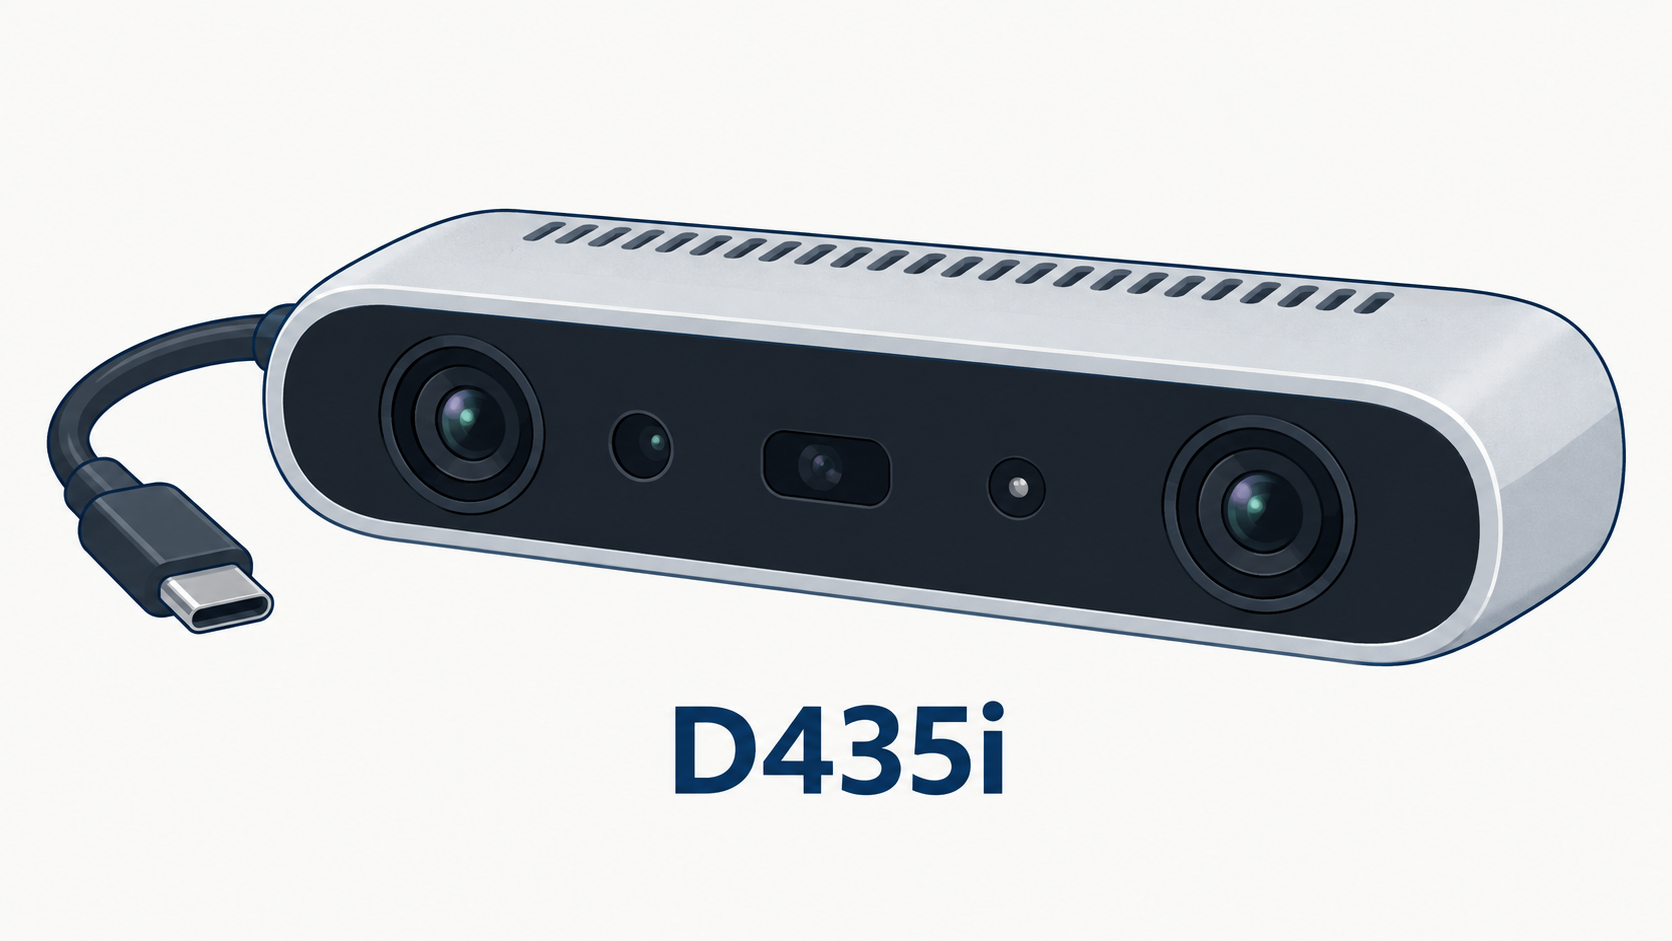
\includegraphics[width=\linewidth,height=.40\textheight,keepaspectratio]{images/P04.png}\par\smallskip
{\small\color{muted}D435i hardware illustration\par}
\end{column}
\end{columns}\vfill
{\centering\color{muted}Owner's operating guide\quad 13 October 2026\par}
\end{frame}

\begin{frame}{Where we are}
\evidence{MEASURED / OPEN}

\pair{Today}{A native ARM64 build produced three usable EuRoC trajectories. D435i recorder and estimator binaries are built; neither has run on this camera.}{Next}{Repair power, preserve/migrate the OS card, qualify data storage, then re-establish N1 $\to$ N2 $\to$ N3 on the new unit.}
\medskip\textbf{Reading route}\par\smallskip
\begin{tabular}{@{}L{80mm}L{30mm}L{48mm}L{22mm}@{}}
Where we are & pp. 2--5 & Today's work & 6--19\\[4pt]
Two programs & 20--28 & Runbook & 29--39\\[4pt]
Tools and sources & 40--42 & Agent tickets & 43--44
\end{tabular}\par\par
\takeaway{All gates remain OPEN. Every command in the runbook is a future instruction.}

\src{[F] sections A--F}{42, 89}
\end{frame}

\begin{frame}{1 / Whole system: today is on the perception side}
\evidence{SOURCE-SUPPORTED / MEASURED / PLANNED}

\road{\node[box] (cam) at (0,0){New D435i\\not yet qualified};
\node[box,fill=teal!10] (pi) at (5,0){Pi 5 / 4 GB\\build + EuRoC};
\node[box] (host) at (10,0){Mac canonical\\evidence + evo};
\draw[flow] (cam)--node[above=8mm,lbl]{local USB}(pi);\draw[flow] (pi)--node[above=8mm,lbl]{copy artifacts}(host);
\node[box,text width=60mm] (ctl) at (5,-2.4){STM32H7\\hard-real-time control / safety};
\draw[flow,dashed] (pi)--node[right,lbl]{PLANNED reviewed interface}(ctl);}
\pair{Ownership}{Acquire locally on the Pi. SSH controls the session; it is not a sensor data path. Keep Mac and Pi checkouts intact.}{Current boundary}{The EuRoC result exercises perception only. It establishes no robot integration, motor safety or controller interface.}

\src{[F] sections A, D; AGENTS.md}{12--15, 41}
\end{frame}

\begin{frame}{1 / Gate ladder: evidence does not transfer sideways}
\evidence{OPEN / MEASURED / PLANNED}

\road{\foreach \x/\n/\t in {0/a/N0 power,4.5/b/N1 identity,9/c/N2 raw,13.5/d/N3 ROS}{\node[box,text width=29mm] (\n) at (\x,0){\t\\OPEN};}
\draw[flow](a)--(b);\draw[flow](b)--(c);\draw[flow](c)--(d);
\node[box,text width=38mm,fill=teal!10] (e) at (0,-2.3){N4A EuRoC\\measured / OPEN};
\node[box,text width=40mm] (f) at (7,-2.3){N4B offline D435i\\built / never run};
\node[box,text width=38mm] (g) at (13,-2.3){N4C live D435i\\built / never run};
\draw[flow](a)--(e);\draw[flow](d.south)--node[above,lbl]{stereo + calibration}(f.north);\draw[flow](f)--(g);}
N4A tests known inputs independently of camera gates. N4B needs the physical gates plus a reviewed stereo extension and calibration. N4C adds live scheduling.
\takeaway{N5 profiling, N6 health and N7 controller integration are still PLANNED.}

\src{[F] sections D--E; Phase A runbook}{42, 58--67}
\end{frame}

\begin{frame}{1 / What changed: treat this as a new unit}
\evidence{MEASURED / OPEN}

\tabtwo{\textbf{Field} & \textbf{Observed 13 October}\\\midrule
Pi / boot storage & Pi 5, 4 GB; Ubuntu 24.04.4; 32 GB microSD, no NVMe\\[5pt]
SDK device serial & \texttt{317422076650}: recorder, ROS serial\_no and gate selection\\[5pt]
ASIC serial & \texttt{327743061057}: separate device identity field\\[5pt]
Firmware-update ID & \texttt{327743061057}: separate observed field\\[5pt]
USB descriptor serial & \texttt{327743061057}: udev / IIO matching\\[5pt]
Firmware / link & 5.17.3.10; reported BMI085; USB 3.2 at 5000 Mbps\\}
\medskip Old SDK \texttt{243322073847}, USB \texttt{251843061466}: September transport/calibration receipts do not qualify this unit.
\takeaway{Fresh N1 must read every identity field; an equal value does not make fields interchangeable.}

\src{[F] sections A--B; ADDENDUM\_CAMERA\_SWAP.md}{14, 46--47}
\end{frame}

\begin{frame}{2 / Platform and power: what actually ran}
\evidence{MEASURED / INFERRED}

\pair{Measured platform}{Pi 5 / 4 GB, kernel 6.8.0-1064-raspi, ROS 2 Jazzy binary, 5 V / 3 A supply. Temporary 4 GB swap helped the build complete.}{Measured warning}{Live under-voltage appeared during load: 46 events during the build; 87 of 178 five-second samples during SLAM runs, or 49\% rounded.}
\medskip A build succeeding under poor power is evidence of compilation, not an eligible performance platform.
\code{vcgencmd get\_throttled\par vcgencmd measure\_temp\par timedatectl status}
\takeaway{Fix the supply first; then record fresh health under the same intended load.}

\src{[F] sections A; N4A power\_window.log}{43--45, 79}
\end{frame}

\begin{frame}{2 / Decode 0x50005: live flags versus history}
\evidence{MEASURED / SOURCE-SUPPORTED}

\tabtwo{\textbf{Bit / mask} & \textbf{Meaning in the runbook}\\\midrule
0 / 0x1 & Under-voltage is occurring now\\[5pt]
2 / 0x4 & Throttling is occurring now\\[5pt]
16 / 0x10000 & Under-voltage has occurred since boot\\[5pt]
18 / 0x40000 & Throttling has occurred since boot\\}
\medskip Thus \texttt{0x50005} contains both live faults and latched history.
\pair{Strict qualification}{Require \texttt{0x0}. Preserve old power logs. After correcting the cause, an owner-chosen reboot starts a fresh observation interval.}{Diagnostic exception}{Explicit latched-only diagnosis can admit \texttt{0x50000}; live bits still stop. Result is OPEN\_DIAGNOSTIC and cannot enter accepted N3.}

\src{[G] active-unit Phase A runbook; [F] sections A}{44, 51}
\end{frame}

\begin{frame}{2 / Why timing is unusable, while accuracy is informative}
\evidence{MEASURED / INFERRED / OPEN}

\road{\node[box] (p) at (0,0){Supply droop};\node[box] (f) at (5,0){CPU throttling};\node[box] (q) at (10,0){Variable CPU\\processing time};\draw[faultflow](p)--(f);\draw[faultflow](f)--(q);}
\pair{Observed duration}{184 s dataset, 282--301 s wall time. Wall time includes vocabulary load, initialization and shutdown; it is not a per-frame tracking benchmark.}{What survives}{Final trajectory error remains measurable against the dataset reference. It supports this algorithm path on MH01, under this recorded run context.}
\medskip No real-time claim follows. Re-measure on stable power; separate startup, per-frame work, queue residence and shutdown. The target 8 GB Pi also needs its own measurements.

\src{[A] REPORT.md; power\_window.log}{78--79, 81--82}
\end{frame}

\begin{frame}{2 / Native build: what the build proved}
\evidence{MEASURED / OPEN}

\road{\node[box] (a) at (0,0){Upstream 4452a3c\\isolated Pi copy};\node[box] (b) at (5,0){Compatibility fixes\\native ARM64};\node[box] (c) at (10,0){Library + examples\\link successfully};\draw[flow](a)--(b);\draw[flow](b)--(c);}
\pair{Build evidence}{Pangolin v0.9.1 built in 178 s. Main library compilation took about 71 min at \texttt{-j2}. Preserve build scripts and Pi-side logs/hashes.}{Meaning}{A usable binary exists for this compiler and dependency set. EuRoC execution is the separate behavioral check; compilation alone cannot establish estimator correctness.}
\takeaway{Upstream acquisition example was unchanged for N4A; the library had three documented compatibility patches.}

\src{[F] sections C; orbslam3-pi-build/build\_orbslam3.sh}{12, 59--60}
\end{frame}

\begin{frame}{2 / Build patch 1: language standard and CPU flags}
\evidence{MEASURED / SOURCE-SUPPORTED}

\pair{Before}{C++11 build settings and \texttt{-march=native} belonged to upstream build assumptions. New compiler/dependency combinations need an explicit compatibility configuration.}{After}{Use C++17 and remove \texttt{-march=native}. Keep the resulting compiler flags in provenance rather than assuming the Mac and Pi build the same code.}
\medskip This is a build configuration change, not a change to stereo features, inertial equations or trajectory evaluation.
\code{\# Read-only inspection of the preserved native build\par cat build/CMakeFiles/ORB\_SLAM3.dir/flags.make}
\takeaway{Record the exact flags and architecture; a successful build does not prove portable binaries.}

\src{[F] sections C; orbslam3-pi-build/build\_orbslam3.sh}{12, 59}
\end{frame}

\begin{frame}{2 / Build patches 2 and 3: two concrete failures}
\evidence{MEASURED / SOURCE-SUPPORTED}

\tabtwo{\textbf{Patch} & \textbf{Failure and bounded fix}\\\midrule
Sophus tests OFF & Sophus unit tests failed with GCC 13 \texttt{-Werror=array-bounds} on aarch64. ORB-SLAM3 uses Sophus headers; skip these third-party tests, retain the failure log.\\[9pt]
\texttt{bool++} to true & C++17 forbids incrementing a bool. Replace \texttt{mnFullBAIdx++} with \texttt{mnFullBAIdx = true}; this preserves the old bool increment result.\\}
\medskip The disabled Sophus tests are a validation limitation. They do not constitute a passing third-party test suite.
\takeaway{Keep patches attached to source identity and build evidence; do not edit canonical upstream to hide the failure.}

\src{[F] sections C; orbslam3-pi-build/build\_orbslam3.sh}{12, 59--60}
\end{frame}

\begin{frame}{2 / Swap: a build aid, not performance evidence}
\evidence{MEASURED / INFERRED}

\pair{Observed}{4 GB RAM plus a temporary 4 GB swapfile. Free RAM fell to about 130 MB during compilation. This is why \texttt{-j2} and swap mattered.}{Inference to test}{An 8 GB Pi may build without swap. That is a hypothesis; no 8 GB build result is present in today's evidence.}
\code{free -h\par swapon --show\par df -B1 /}
\medskip Build pressure and runtime pressure are different workloads. N4A peak RSS was 823--828 MiB; neither that figure nor the swapfile size is the total system memory requirement.
\takeaway{Log RAM, swap use and storage headroom; avoid extra flash writes during capture.}

\src{[F] sections C; [A] REPORT.md}{44, 79}
\end{frame}

\begin{frame}{2 / EuRoC MH01: known input before camera adaptation}
\evidence{MEASURED / SOURCE-SUPPORTED}

\road{\node[box] (a) at (0,0){Stereo gray\\20 Hz};\node[box] (b) at (5,0){Drone IMU\\200 Hz};\node[box] (c) at (10,0){Independent reference\\ground truth};
\node[box,text width=130mm,fill=teal!10] (d) at (5,-2){MH\_01\_easy: machine hall / public ETH dataset\\184 s, 3,682 stereo frames in the session inventory};
\draw[flow](a)--(d);\draw[flow](b)--(d);\draw[flow](c)--(d);}
\medskip The dataset supplies images, motion samples, timestamps and its own settings. Our D435i is absent from this test, so its USB link and calibration cannot cause these input failures.
\takeaway{First establish that the native estimator can use known, calibrated input.}

\src{[A] REPORT.md; ETH EuRoC dataset; upstream EuRoC.yaml}{59}
\end{frame}

\begin{frame}{2 / Ground truth: an independently measured answer}
\evidence{SOURCE-SUPPORTED / MEASURED}

Ground truth is the reference pose trajectory used to score the estimate. It is obtained with external measurement equipment, not by trusting ORB-SLAM3's own map.
\pair{EuRoC reference}{Machine-hall data uses laser-tracker position measurements; the dataset provides processed state ground truth. Vicon-room sequences use motion capture. Do not claim MH01 has Vicon measurements.}{Evaluation here}{Use \texttt{state\_groundtruth\_estimate0/data.csv}, convert to TUM, and compare body/IMU poses in the same frame convention and time units.}
\medskip A hand-carried D435i take has no external ground truth in the current plan. A closed loop or a plausible path cannot substitute for one.
\takeaway{Ground truth still has coverage, timing and measurement uncertainty to document.}

\src{[A] REPORT.md; Campos et al., accepted paper, EuRoC discussion}{59, 75, 77}
\end{frame}

\begin{frame}{2 / ATE: remove the arbitrary origin, keep scale}
\evidence{SOURCE-SUPPORTED / MEASURED method}

Let $\hat p_i$ be an estimated body position and $p_i$ its time-associated reference position. Fit one rigid transform to the whole accepted trajectory:
\[
(R^*,t^*)=\arg\min_{R\in SO(3),\,t}\sum_{i=1}^{n}\|R\hat p_i+t-p_i\|^2.
\]
Then $r_i=R^*\hat p_i+t^*-p_i$ and
\[\mathrm{ATE}_{\mathrm{RMSE}}=\sqrt{\frac{1}{n}\sum_{i=1}^{n}\|r_i\|^2}.\]
\medskip SE(3) means rotation + translation only. Stereo-inertial has metric scale; adding scale fitting (Sim(3)) would conceal scale error.
\takeaway{Alignment removes coordinate choice; the remaining residuals measure position mismatch.}

\src{[A] REPORT.md; Campos et al., accepted paper, Sec. VII}{75}
\end{frame}

\begin{frame}{2 / ATE alignment: schematic before and after}
\evidence{SOURCE-SUPPORTED / ASSUMED schematic}

\begin{center}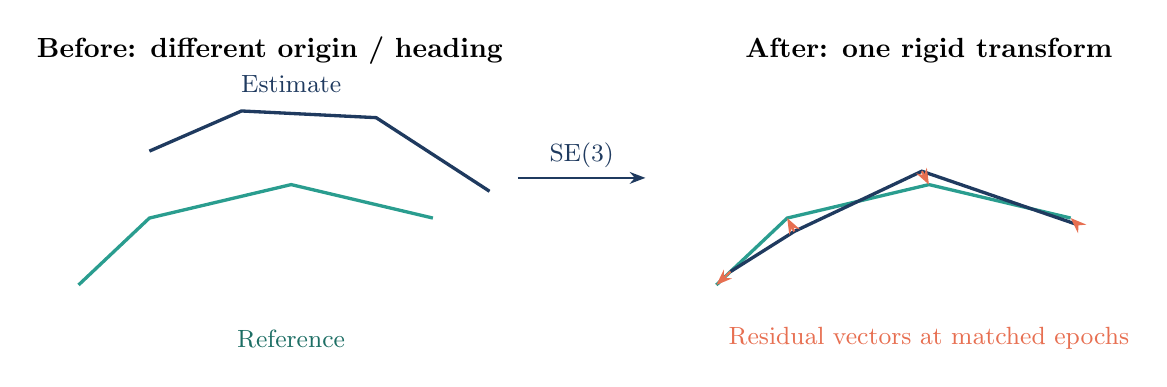
\begin{tikzpicture}[x=.9cm,y=.85cm,font=\small]
\node[font=\normalsize\bfseries] at (2.7,3.5){Before: different origin / heading};
\node[font=\normalsize\bfseries] at (12,3.5){After: one rigid transform};
\draw[teal,very thick] (0,0)--(1,1)--(3,1.5)--(5,1);
\draw[navy,very thick] (1,2)--(2.3,2.6)--(4.2,2.5)--(5.8,1.4);
\draw[flow] (6.2,1.6)--node[above]{SE(3)}(8,1.6);
\draw[teal,very thick] (9,0)--(10,1)--(12,1.5)--(14,1);
\draw[navy,very thick] (9.2,.2)--(10.1,.8)--(11.9,1.7)--(14.1,.9);
\foreach \a/\b/\c/\d in {9.2/.2/9/0,10.1/.8/10/1,11.9/1.7/12/1.5,14.1/.9/14/1}{\draw[faultflow](\a,\b)--(\c,\d);}
\node[text=teal!70!black] at (3,-.8){Reference};\node[text=navy] at (3,3){Estimate};
\node[text=fault] at (12,-.8){Residual vectors at matched epochs};
\end{tikzpicture}\end{center}
\medskip No axes or numerical errors are implied by this drawing. ATE uses all accepted matched positions, not just the four illustrated points.
\takeaway{No scale change is permitted; residual lengths are combined by RMS.}

\src{[A] REPORT.md evaluation protocol}{75}
\end{frame}

\begin{frame}{2 / evo: reproduce the score and distinguish RPE}
\evidence{MEASURED ATE protocol / CALCULATED RPE}

\begin{tabular}{@{}L{27mm}L{70mm}L{70mm}@{}}\toprule
\textbf{Run} & \textbf{RPE trans. RMSE (m)} & \textbf{RPE rot. RMSE (deg)}\\\midrule
1 & 0.013295 & 0.076464\\[5pt]
2 & 0.013559 & 0.076776\\[5pt]
3 & 0.014021 & 0.074883\\\bottomrule\end{tabular}\par
\medskip SE(3); shared EuRoC clock assumed, offset 0 s; association tolerance 0.02 s (3,639 matched pose pairs per run).
\medskip One endpoint per eligible start: first later reference pose $\geq1$ s later; no interpolation. These are \texttt{traj\_eval.py} results; its pair policy differs from evo's RPE filters.
\takeaway{About 1.3 cm RPE over 1 s describes local drift; ATE scores the aligned global path.}
\note{Evidence: slides\_course/qa/n4a-traj-eval-summary.md; tools/trajectory\_eval/README.md. CALCULATED using traj\_eval.py from claude/project-thread-upkfjv, commit d3f9540, PR 2; tool not yet merged. Tool validation passed per its README, not rerun by this deck task. Flags: --t-max-diff 0.02 --t-offset 0 --align-both --rotation-ate --rpe-delta 1 --rpe-unit s. Shared EuRoC clock assumed; offset zero; active body-to-world poses in imu\_body, metres. 3,639 timestamp-associated pose pairs per run. For each eligible start, choose the first later reference timestamp at least 1 s later; no interpolation. SE(3) rigid alignment cancels in RPE. The tool's SE(3) ATE reproduces saved evo scores; its RPE pair policy differs from evo filters. Sim(3) additionally fits scale and is diagnostic, not the stereo-inertial paper comparator. Does not establish frames, extrinsics, synchronization, sensor readiness or gate PASS. No new camera, Pi or ORB execution.}
\src{C: qa/n4a-traj-eval-summary.md; d3f9540 / PR 2, unmerged}{76, 80}
\end{frame}

\begin{frame}{2 / Three runs: score range, not a single best screenshot}
\evidence{MEASURED / SOURCE-SUPPORTED / CALCULATED}

\begin{tabular}{@{}L{27mm}L{36mm}L{32mm}L{30mm}L{40mm}@{}}\toprule
\textbf{Run} & \textbf{ATE RMSE} & \textbf{ATE max} & \textbf{Wall time} & \textbf{Peak RSS}\\\midrule
1 & 0.0415 m & 0.081 m & 301 s & 823 MiB\\[5pt]
2 & 0.0368 m & 0.076 m & 282 s & 828 MiB\\[5pt]
3 & 0.0416 m & 0.088 m & 284 s & 828 MiB\\\bottomrule\end{tabular}\par
\medskip All three: one map, no resets, IMU initialized, exit 0; 3,678 output poses. Mean RMSE about 0.040 m; range 0.0368--0.0416 m.
\medskip \textbf{Verified paper comparator: 0.036 m.} Campos et al., Table II, MH01 stereo-inertial; median of ten runs, processed GT, SE(3). Our three-run mean is a different statistic and protocol equivalence is not fully established.
\takeaway{Similar error magnitude is useful baseline evidence, not a formal reproduction or gate acceptance.}

\src{[A] REPORT.md; \href{https://arxiv.org/pdf/2007.11898}{Campos et al., accepted paper, Table II}}{60, 66, 80}
\end{frame}

\begin{frame}{2 / Variation and gate status: what N4A establishes}
\evidence{MEASURED / INFERRED / OPEN}

\pair{Supported by these trials}{The native ARM64 estimator and compatibility fixes produce finite, initialized trajectories on MH01 with centimeter-scale ATE near the published comparator.}{Still unproven}{D435i geometry/noise/clock, physical transport, other sequences and healthy real-time performance. N4A RPE is now CALCULATED (p. 17). Numeric acceptance budgets remain OPEN.}
\medskip Mapping and loop-closing threads can execute in different orders. Identical input need not produce identical keyframes; observed counts were 126 / 126 / 129. Scheduling is a plausible explanation, not a measured cause of the score variation.
\medskip Pi UTC labels were about 80 min behind before NTP was restored near 09:45Z. Retain the offset note; do not align Mac/Pi logs by uncorrected labels.
\takeaway{N4A remains OPEN; power and protocol/budget review are unresolved.}

\src{[A] REPORT.md; [F] sections A, D}{60, 67, 79}
\end{frame}

\begin{frame}{3 / Two programs: record once, run the estimator later}
\evidence{MEASURED build / OPEN execution}

\pair{\texttt{d435i\_record}}{An acquisition utility. Uses librealsense directly, records left/right IR and raw gyro/accel, and writes a timestamp audit. It does not run SLAM.}{\texttt{stereo\_inertial\_realsense\_D435i}}{A patched upstream input example. Feeds stereo images and associated IMU samples to ORB-SLAM3, then saves body and keyframe trajectories.}
\medskip Built bundle: \texttt{\detokenize{~/wbr-runtime/n4b-20261013T080913Z/bin/}}. Linkage was reported clean. Neither binary has been exercised with this camera or a real recording.
\takeaway{Run one camera-owning process at a time. A clean link is not a validated input path.}

\src{[F] sections E; [B] README.md}{15, 61--65}
\end{frame}

\begin{frame}{3 / Recorder profile: stereo development adds bandwidth}
\evidence{SOURCE-SUPPORTED / PLANNED acquisition}

\tabtwo{\textbf{Stream} & \textbf{Explicit selected profile}\\\midrule
IR1 and IR2 & Left/right infrared, each 640$\times$480, Y8, 30 Hz\\[6pt]
Gyroscope & Raw XYZ angular velocity, 200 Hz\\[6pt]
Accelerometer & Raw XYZ acceleration, 100 Hz\\[6pt]
Excluded & No depth/RGB; no rate fallback; no combined ROS IMU\\}
\medskip This is the N4 development profile. Strict N2 stays IR1-only at 15 Hz with gyro/200 and accel/100. N3 preserves that baseline before the reviewed stereo extension.
\takeaway{Selecting a supported profile does not measure actual delivery under recording load.}

\src{[B] d435i\_rs.h; n4b\_plan.md}{9, 48--51, 58}
\end{frame}

\begin{frame}{3 / Emitter OFF: features must belong to the scene}
\evidence{SOURCE-SUPPORTED / PLANNED readback}

\road{\node[box] (a) at (0,0){Projected dots\\move with projector};\node[box] (b) at (5,0){Static scene texture\\belongs to scene};\node[box,fill=teal!10] (c) at (10,0){ORB features\\track real structure};\draw[faultflow,dashed](a.north)--++(0,.5)-|(c.north);\draw[flow](b)--(c);}
\medskip Projected texture has view-dependent behavior and can confuse feature identity between cameras and over time. Both live programs set the emitter OFF and read the option back before streaming.
\pair{Prepare scene}{Diffuse light, textured static objects, short exposure and modest motion; inspect IR for blur and saturation.}{Preserve context}{Record exposure metadata and motion-correction/global-time settings. Emitter OFF alone does not qualify image quality or timestamps.}

\src{[B] n4b\_plan.md; d435i\_rs.h}{9, 29--30, 57}
\end{frame}

\begin{frame}{3 / Recorder outputs: timestamps are evidence, not truth}
\evidence{SOURCE-SUPPORTED / OPEN}

\pair{One new take directory}{\texttt{stereo\_imu.db3}: SDK recording.\par \texttt{timestamps.csv}: full-precision stream/time/IMU audit.\par \texttt{sdk.log}: unfiltered SDK messages.}{What to reconcile}{Stored decoded counts versus callbacks; image pixels and strides; timestamp domains, frame steps, boundaries and left/right pairing. Count differences must be explained.}
\medskip The recorder uses device timestamps. Host arrival/steady time serves a separate audit purpose; it cannot silently replace sensor time in SLAM.
\medskip Local source now names \texttt{.db3}; older preparation prose still says \texttt{.bag}. Use the built-binary/source hash and actual finalized output. Confirm SDK playback compatibility rather than assuming an ordinary ROS topic bag.
\takeaway{Normal stop finalizes the file. Hash it before playback and keep every failed take.}

\src{[B] d435i\_record.cpp; n4b\_plan.md}{24--26, 63}
\end{frame}

\begin{frame}{3 / Storage arithmetic: 18.4 MB/s is only the floor}
\evidence{CALCULATED / MEASURED history / OPEN}

\[
2\times640\times480\times1\times30
=18{,}432{,}000\ \mathrm{B/s}=18.432\ \mathrm{MB/s}.
\]
Pixels alone: 1.106 GB/min; a 90 s take is 1.659 GB. Raw motion floats add 216 kB/min before timestamps, metadata, serialization and CSV.
\pair{Historical warning}{September card probe about 19 MB/s, worst about 17 MB/s: too little margin against this stereo payload. Today's free space must be rechecked after build/swap.}{Planning allowance}{Preparation proposes 1.5 GB/min provisionally. Actual finalized size, sustained/peak writes and backlog are still UNKNOWN. Card labels are not measurement evidence.}
\takeaway{GB-scale bags require separately qualified storage. The larger OS card does not satisfy that prerequisite by capacity alone.}

\src{[B] n4b\_plan.md; [F] sections F}{18, 56}
\end{frame}

\begin{frame}{3 / Patched estimator: one executable, two modes}
\evidence{SOURCE-SUPPORTED / MEASURED build / OPEN}

\code{\# N4B: immutable recording, playback is not real-time\par \$WBR\_SLAM VOCAB YAML run01 --bag TAKE.db3 --no-viewer\par \# N4C: same vocabulary and YAML, direct live source\par \$WBR\_SLAM VOCAB YAML live01 --no-viewer}
\pair{\texttt{--bag FILE}}{File-only device resolution, no loop, preserved source stamps. Disable real-time playback before start; allow processing to finish without dropping to wall-clock pacing.}{\texttt{--no-viewer}}{Disable the GUI. Pangolin remains a linked dependency; headless behavior does not eliminate its build requirement.}
\takeaway{These are future command shapes. N4B isolates input/calibration; N4C adds live overload and source-age questions.}

\src{[B] stereo\_inertial\_d435i\_file.patch}{61--65}
\end{frame}

\begin{frame}{3 / IMU patch: interpolate within valid brackets}
\evidence{SOURCE-SUPPORTED / synthetic-tested / OPEN SDK behavior}

\begin{center}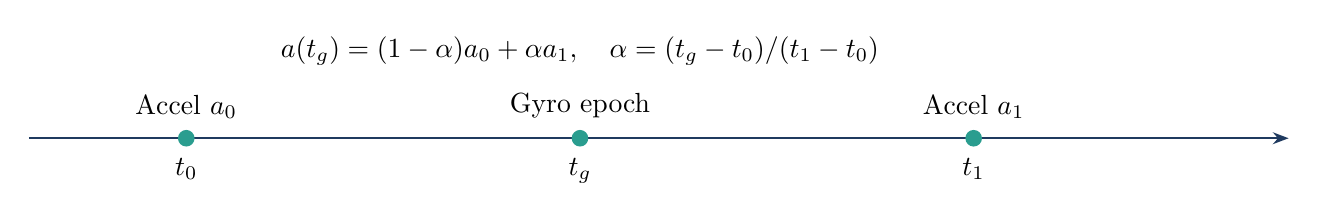
\begin{tikzpicture}[x=1cm,y=.65cm,font=\normalsize]
\draw[flow](0,0)--(16,0);\foreach \x/\t in {2/t_0,7/t_g,12/t_1}{\fill[teal](\x,0) circle(3pt);\node[below] at (\x,-.2){$\t$};}
\node[above] at (2,.2){Accel $a_0$};\node[above] at (7,.2){Gyro epoch};\node[above] at (12,.2){Accel $a_1$};
\node at (7,1.7){$a(t_g)=(1-\alpha)a_0+\alpha a_1,\quad \alpha=(t_g-t_0)/(t_1-t_0)$};
\end{tikzpicture}\end{center}
\medskip Fix upstream interpolation overwrite; send each gyro once with bracketed accel. Retain the endpoint at/after an image for preintegration. Reject nonfinite, duplicate/backward samples and interior motion gaps over 50 ms; never extrapolate.
\medskip Explicitly count uncovered startup/EOF images and samples. A gyro-grid input at 200 Hz still contains measured accel at 100 Hz.
\takeaway{Synthetic tests verify association logic only; real-file EOF/callback behavior remains OPEN.}

\src{[B] d435i\_input.h; verification.md}{35, 38}
\end{frame}

\begin{frame}{3 / End-to-end path: offline before live}
\evidence{SOURCE-SUPPORTED / PLANNED execution}

\begin{center}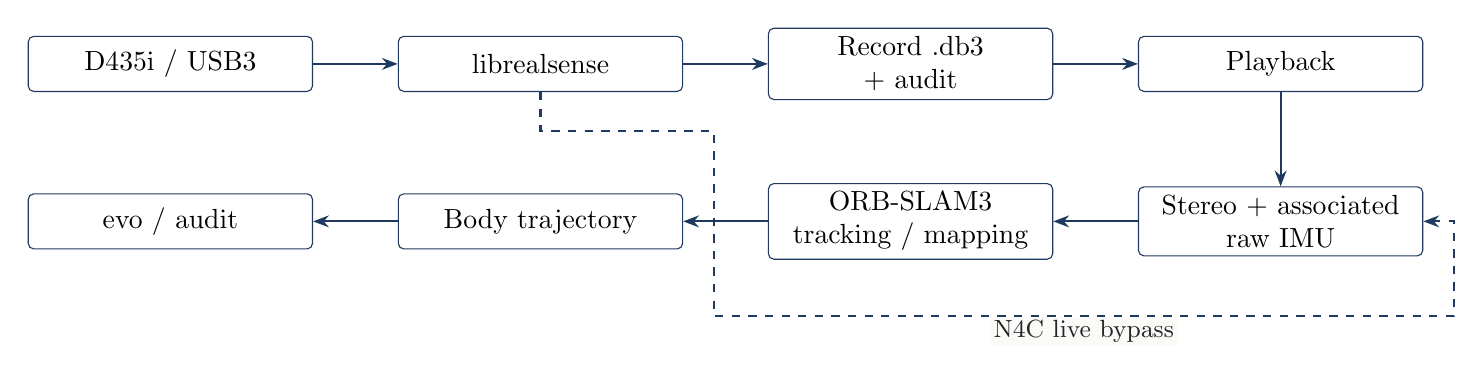
\begin{tikzpicture}[box/.append style={font=\normalsize,text width=34mm},node distance=9mm]
\node[box](a) at (0,0){D435i / USB3};\node[box](b) at (4.7,0){librealsense};\node[box](c) at (9.4,0){Record .db3\\+ audit};\node[box](d) at (14.1,0){Playback};
\node[box](e) at (14.1,-2){Stereo + associated\\raw IMU};\node[box](f) at (9.4,-2){ORB-SLAM3\\tracking / mapping};\node[box](g) at (4.7,-2){Body trajectory};\node[box](h) at (0,-2){evo / audit};
\draw[flow](a)--(b);\draw[flow](b)--(c);\draw[flow](c)--(d);\draw[flow](d)--(e);\draw[flow](e)--(f);\draw[flow](f)--(g);\draw[flow](g)--(h);
\draw[flow,dashed](b.south)--(4.7,-.85)--(6.9,-.85)--(6.9,-3.2)--node[below,lbl]{N4C live bypass}(16.3,-3.2)--(16.3,-2)--(e.east);\end{tikzpicture}\end{center}
\medskip Frozen data enables repeated diagnosis without repeating hand motion. The eight-pair image queue owns pixels; playback waits for space, while live overload fails explicitly. Neither mode permits silent latest-frame overwrite.
\takeaway{Repeated offline runs can still vary because mapping is threaded. Preserve all outputs.}

\src{[B] n4b\_plan.md; patch}{17, 32--34, 63}
\end{frame}

\begin{frame}{3 / Configuration register: readback versus calibration}
\evidence{MEASURED readback / ASSUMED noise / OPEN}

\tabtwo{\textbf{Quantity} & \textbf{Candidate YAML / confidence}\\\midrule
IR intrinsics & $f_x=f_y=386.95$, $c_x=321.03$, $c_y=241.04$ px at 640$\times$480; SDK rectified readback\\[5pt]
Stereo baseline & $b=0.0499126$ m; positive magnitude of IR1$\to$IR2 translation\\[5pt]
\texttt{IMU.T\_b\_c1} & Camera$\to$gyro/body, identity rotation; $t=(-5.52,+5.10,+11.74)$ mm; nominal factory geometry\\[5pt]
IMU noise / walks & $10^{-3},10^{-2},10^{-6},10^{-4}$ in upstream key order; ASSUMED, not unit measurements\\}
\medskip Keep the reported ``IMU Calibration is not available'' warning. Fresh SDK logs must establish its occurrence on this unit; old warning logs are not new-unit evidence.
\takeaway{Noise, bias/scale, actual alignment and camera--IMU time offset remain unqualified. Built binaries have never run here.}

\src{[B] calibration\_notes.md; candidate YAML; [F] sections E}{23, 28--31, 36--37, 85}
\end{frame}

\begin{frame}{4 / Runbook entry: prepare a bounded session}
\evidence{PLANNED / OPEN}

\pair{Before any execution}{User must explicitly say CAMERA AVAILABLE before camera-dependent commands or ORB execution. Capture locally on Pi; use a verified runtime bundle, fresh evidence directory and exact active-unit selection.}{Order of decisions}{Power $\to$ OS migration $\to$ separate data storage $\to$ N1 $\to$ N2 $\to$ N3 $\to$ stereo development take $\to$ N4B $\to$ calibration $\to$ qualified offline review $\to$ N4C $\to$ profiling.}
\code{\# Alias declarations; resolve actual bundle paths first\par export WBR\_BUNDLE="VERIFIED\_RUNTIME\_BUNDLE"\par export WBR\_SLAM=\$WBR\_BUNDLE/bin/stereo\_inertial\_realsense\_D435i\par export WBR\_DATA="QUALIFIED\_SEPARATE\_DATA\_MOUNT"}
\takeaway{The next pages specify acceptance conditions; they do not report PASS. Stop on nonzero exit and inspect evidence before progressing.}

\src{[G] active-unit Phase A runbook; [B] n4b\_plan.md}{42--67, 72}
\end{frame}

\begin{frame}{4 / Step 1: repair power and establish N0 eligibility}
\evidence{PLANNED / OPEN}

\textbf{Goal / tool:} stable supply and cooling; \texttt{vcgencmd}, inventory and UTC service. Ordered supply: 5.1 V / 5 A; verify the physical label/cable.
\code{python3 platform\_inspect.py > NEW-inventory.json\par vcgencmd get\_throttled\par vcgencmd measure\_temp\par timedatectl status}
\pair{Expected / acceptance}{ARM64 Ubuntu 24.04, Jazzy, synchronized UTC, flags \texttt{0x0}, temperature $<75\,^{\circ}$C, MemAvailable $\ge512$ MiB. Repeat health under intended load.}{Failure $\to$ inspect}{Live voltage bits $\to$ supply/cable/connectors. Heat $\to$ cooling. Latched bits $\to$ retain history, correct cause, owner-chosen reboot then fresh evidence; do not mask flags.}
\takeaway{The supply rating is a plan. Fresh healthy observations determine eligibility.}

\src{[G] active-unit Phase A runbook; [F] sections A}{43--45}
\end{frame}

\begin{frame}{4 / Step 2: migrate the OS card, qualify data separately}
\evidence{PLANNED / OPEN / CALCULATED capacity}

\textbf{Goal / tool:} image the 32 GB card on Mac, write the verified clone to 128 GB V30/A2, grow root; keep the original card as rollback.
\code{diskutil list \quad\# Mac: inspect disks before a reviewed clone\par lsblk -f; findmnt -T /; df -B1 / \quad\# Pi after migration}
\pair{Expected / acceptance}{Image hash and readback; original retained; clone boots with files/versions intact, root size checked and fresh N0.}{Failure $\to$ inspect}{Wrong root size $\to$ growth procedure; boot/files missing $\to$ image/hash and disk identity. Retain the original.}
\medskip About 95 GB data capacity is arithmetic only. Large bags require a separate qualified mount: \texttt{storage\_qualify.py} with inspected UUID/device, then fresh N1. See [G] for the full storage contract.

\src{[F] sections F; [G] active-unit Phase A runbook storage section}{18, 45, 56}
\end{frame}

\begin{frame}{4 / Step 3: fresh N1 on the new D435i}
\evidence{PLANNED / OPEN}

\textbf{Goal / tool:} verify camera's own USB branch, normal-user permissions, device identity and healthy platform; \texttt{n1\_precheck.py}.
\code{python3 n1\_precheck.py --camera-available \textbackslash{}\par \quad --direct-cable-confirmed --output "\$WBR\_RUN/n1"}
\pair{Expected / acceptance}{Sealed \texttt{result.json}, own branch $\ge5000$M, direct cable, video/HID/IIO access, all four identity fields, firmware readback; strict health. Receipt matches host/boot and is at most two hours old.}{Failure $\to$ inspect}{480M $\to$ cable/port/hub, stop before SDK. Motion permission denied $\to$ serial-matched HID/IIO controls. Wrong serial $\to$ SDK versus descriptor selection. No broad permissions or firmware update.}
\takeaway{N1 previously stopped at the clock prerequisite. NTP repair alone does not produce a new N1 receipt.}

\src{[G] active-unit Phase A runbook; [F] sections B, E}{46--47}
\end{frame}

\begin{frame}{4 / Step 4: N2 strict raw transport and mandatory soak}
\evidence{PLANNED / OPEN}

\textbf{Goal / tool:} prove native delivery before ROS/SLAM; \texttt{phase\_gate.py}. IR1 Y8 640$\times$480/15, gyro/200, accel/100, unchanged.
\code{python3 phase\_gate.py n2 --camera-available --seconds 20 \textbackslash{}\par \quad --n1-result "\$WBR\_RUN/n1/result.json" --output "\$WBR\_RUN/smoke"\par \# Then 105 s, then 300 s; chain --previous sealed receipts}
\pair{Expected / acceptance}{Raw CSV/logs, health and images. IR 14.25--15.75 Hz; gyro 190--210; accel 95--105. Image gap $\le0.20$ s, motion $\le0.05$ s; positive stamp/frame steps, no missing image numbers.}{Failure $\to$ inspect}{Rate/gap $\to$ CSV boundaries; USB reset $\to$ journal; voltage $\to$ supply. Review images and warning; \texttt{accept-n2} requires actual review.json.}
\takeaway{The 300 s raw soak is mandatory. A 105 s run or OPEN\_DIAGNOSTIC cannot replace acceptance.}

\src{[G] active-unit Phase A runbook N2 sections}{48--52, 72}
\end{frame}

\begin{frame}{4 / Step 5: N3 ROS record and isolated replay}
\evidence{PLANNED / OPEN wrapper state}

\textbf{Goal / tools:} qualify ROS delivery/record/replay with realsense-ros, rosbag2 and observers. Verify installed wrapper; 4.58.4 is only the prepared target.
\code{python3 n3\_record.py --camera-available --n1-result N1.json \textbackslash{}\par \quad --n2-result N2.json --storage-result STORAGE.json \textbackslash{}\par \quad --bag QUALIFIED/NEW\_BAG --seconds 20 --output RECORD\par python3 n3\_bag.py replay QUALIFIED/NEW\_BAG \textbackslash{}\par \quad --record-result RECORD/result.json --live-domain 42 \textbackslash{}\par \quad --replay-domain 43 --output-dir REPLAY}
\medskip \textbf{Expected / acceptance:} 60 s live observer, N2 rate/gap bands under load; exact topics/types/frames/context and finalized metadata. Stop live source; replay counts and decoded payload hashes must match.
\medskip \textbf{Failure $\to$ inspect:} context/QoS $\to$ version/readback; replay contamination $\to$ processes/domains. Review stereo separately.

\src{[G] active-unit Phase A runbook N3 sections}{53--58}
\end{frame}

\begin{frame}{4 / Step 6: first guided stereo take, 60--90 seconds}
\evidence{PLANNED development / OPEN qualification}

\begin{center}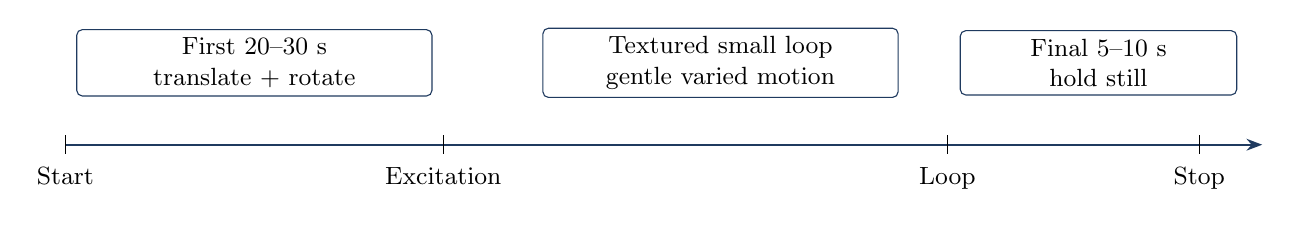
\begin{tikzpicture}[x=.16cm,y=.8cm,font=\small]
\draw[flow](0,0)--(95,0);\foreach \x/\t in {0/Start,30/Excitation,70/Loop,90/Stop}{\draw(\x,.15)--(\x,-.15);\node[below] at(\x,-.2){\t};}
\node[box,text width=43mm] at(15,1.3){First 20--30 s\\translate + rotate};\node[box,text width=43mm] at(52,1.3){Textured small loop\\gentle varied motion};\node[box,text width=33mm] at(82,1.3){Final 5--10 s\\hold still};\end{tikzpicture}\end{center}
\medskip \textbf{Recipe:} translate 10--30 cm in all axes with $\pm15$--$30^\circ$ rotations, keep texture visible, avoid shocks/blur. The timing bars are approximate recipe stages, not a measured trajectory.
\code{\# Recorder creates TAKE exclusively; parent is on qualified storage\par \$WBR\_BUNDLE/bin/d435i\_record "\$WBR\_TAKE" 90}
\medskip \textbf{Expected / acceptance:} all four callback streams, finalized .db3 + CSV + raw SDK logs, emitter readback OFF; decoded counts/pixels/stamps reconciled and actual 30 Hz stereo assessed. ``OPEN: recorded'' is not acceptance. Missing streams/error $\to$ raw logs/profile/storage.

\src{[B] n4b\_plan.md; d435i\_record.cpp}{30, 35, 58, 62}
\end{frame}

\begin{frame}{4 / Step 7: offline N4B run, then evaluate honestly}
\evidence{PLANNED / OPEN / no external GT for hand take}

\textbf{Goal / tool:} diagnose the fixed take before live; patched example plus trajectory/timestamp audit.
\code{\$WBR\_SLAM VOCAB YAML run01 \textbackslash{}\par \quad --bag "\$WBR\_TAKE/stereo\_imu.db3" --no-viewer}
\pair{Expected / acceptance}{``IMU initialized''; finite ordered poses, map/reset timeline and input/rejection audit. One map/no resets is a development goal; numeric budgets remain OPEN.}{Failure $\to$ inspect}{``Not enough motion... Reseting'' $\to$ excitation/time/calibration. Coverage timeout $\to$ brackets; vertical disparity $\to$ rectification; empty poses $\to$ raw logs.}
\medskip Repeat the hashed take/config. Without independent ground truth, report continuity/repeatability and closure discrepancy; ATE is unavailable.

\src{[B] n4b\_plan.md; patch}{62--63, 67, 75--77}
\end{frame}

\begin{frame}{4 / Step 8: calibrate camera--IMU geometry and time}
\evidence{PLANNED / SOURCE-SUPPORTED / OPEN tool integration}

\textbf{Goal / tool:} estimate spatial transform and time offset with Kalibr; plan a fixed Aprilgrid and excite all axes under good light.
\code{\# Future compatible Kalibr environment, not an installed Pi command\par kalibr\_calibrate\_imu\_camera --bag CALIBRATION.bag \textbackslash{}\par \quad --cam camchain.yaml --imu imu.yaml --target aprilgrid.yaml}
\medskip \textbf{Expected / acceptance:} report PDF, result text and camchain-imucam YAML; review residuals, coverage and holdout behavior. Verify transform direction/units and offset sign once. Approved residual budgets are still OPEN.
\medskip \textbf{Failure $\to$ inspect:} poor fit $\to$ blur/target coverage/time jitter/IMU model before tuning. Kalibr expects a compatible ROS bag; SDK .db3 import and topic/model compatibility need a reviewed, lossless conversion path. No converter is claimed ready.
\takeaway{Resolve IMU intrinsics/noise too. Then repeat offline N4B with frozen accepted calibration before any N4C qualification.}

\src{[B] calibration\_notes.md; \href{https://github.com/ethz-asl/kalibr/wiki/camera-imu-calibration}{Kalibr primary documentation}}{28--31, 62, 85}
\end{frame}

\begin{frame}{4 / Step 9: measure IMU noise with Allan deviation}
\evidence{PLANNED / ASSUMED current YAML / OPEN}

\textbf{Goal / tool:} replace example noise densities and bias walks with unit evidence. Candidate: \texttt{allan\_variance\_ros}; import/build compatibility has not been qualified.
\code{TOOL --help \quad\# Pin and review the selected interface first\par TOOL STATIONARY\_RAW\_IMU CONFIG OUTPUT}
\pair{Expected / acceptance}{Stationary full-precision six-axis data, stamps/units/temperature and no clipping/gaps; deviation curves + density/walk fits. Duration from required averaging times, normally hours.}{Failure $\to$ inspect}{Curve artifacts $\to$ stamps/gaps/motion; weak long-time fit $\to$ duration. Review units; avoid double discretization in ORB.}
\medskip The hand take is too short for slow bias. Duration and fit acceptance need review. Zero SDK variance does not mean noiseless hardware.

\src{[B] calibration\_notes.md; Kalibr IMU noise guidance}{31, 37, 85}
\end{frame}

\begin{frame}{4 / Step 10: live N4C, then profile N5}
\evidence{PLANNED / OPEN thresholds}

\textbf{Goal / tools:} retain the accepted offline configuration while testing live scheduling; same example, gate observers and \texttt{vcgencmd}.
\code{\$WBR\_SLAM VOCAB QUALIFIED.yaml live01 --no-viewer\par vcgencmd get\_throttled \quad\# Alongside health sampling}
\pair{Expected / acceptance}{Finite tracking + state events, source/host epochs; pairing, drop/overflow, queues/source age and CPU/RSS/thermal/power logs. Accuracy/latency/loss budgets need approval.}{Failure $\to$ inspect}{Live-only overflow $\to$ queues; growing delay $\to$ backlog; loss in both modes $\to$ input/calibration. Under-voltage $\to$ stop and repair.}
\medskip N5 separates startup, tracking, queues and shutdown; report p50/p95/max with clock definitions. Missing counters remain unavailable. Measure healthy 4 GB and target 8 GB separately.

\src{[B] n4b\_plan.md; course N4C/N5 tables}{64--67, 78--82}
\end{frame}

\begin{frame}{5 / Tool map: platform, transport and recording}
\evidence{MEASURED components / PLANNED physical use / OPEN wrapper}

\begin{tabular}{@{}L{39mm}L{90mm}L{55mm}@{}}\toprule
\textbf{Tool} & \textbf{Job / step} & \textbf{Status here}\\\midrule
vcgencmd / journal & Power, temperature, kernel faults; N0--N5 & Used in saved evidence\\[5pt]
librealsense & SDK enumeration, raw device/file input; N1/N2/N4 & SDK present; new path unrun\\[5pt]
Gate utilities & Sealed N1/N2/N3 checks, health and replay & Offline tests; gates OPEN\\[5pt]
realsense-ros & ROS topics, parameters, frame/context; N3 & Installed state to verify\\[5pt]
rosbag2 & ROS bag record/info/play; N3 & Future qualification\\[5pt]
d435i\_record & SDK stereo/motion .db3 + audit; first take & Built, never run\\[5pt]
Storage qualifier & Sustained writes/hash readback; data entry & Separate mount PLANNED\\\bottomrule\end{tabular}\par
\takeaway{SDK recording and N3 ROS recording are distinct paths; they have different inventories and qualification evidence.}

\src{[F] sections A--E; [G] active-unit Phase A runbook}{9--11, 18, 46--58, 72}
\end{frame}

\begin{frame}{5 / Tool map: estimation, scoring and calibration}
\evidence{MEASURED baseline / ASSUMED config / PLANNED calibration}

\begin{tabular}{@{}L{42mm}L{89mm}L{53mm}@{}}\toprule
\textbf{Tool} & \textbf{Job / step} & \textbf{Status here}\\\midrule
ORB-SLAM3 & Features + inertial tracking/mapping; N4 & EuRoC ran; D435i unrun\\[5pt]
Pangolin & Upstream visualization/build dependency & v0.9.1 built; headless link\\[5pt]
Patched D435i example & Shared offline/live association; N4B/C & Built; SDK behavior OPEN\\[5pt]
evo / traj\_eval & Global ATE / local RPE; N4A/N5 & ATE used; RPE CALCULATED\\[5pt]
Kalibr & Camera--IMU transform/time + reports & PLANNED integration\\[5pt]
Allan-variance tool & Noise/walk from stationary IMU & PLANNED tool selection\\[5pt]
Hashes / manifests & Bind source, config, input and results & Required every stage\\\bottomrule\end{tabular}\par
\takeaway{Choose the next tool from the unresolved question: delivery, input association, calibration or scheduling.}

\src{[F] sections C--E; [B] calibration\_notes.md}{12, 32--38, 67, 75--79, 85}
\end{frame}

\begin{frame}{5 / Source key: how to verify each claim}
\evidence{SOURCE-SUPPORTED / OPEN evidence limitations}
\tabtwo{\textbf{Key} & \textbf{Repository source (all under experiments/ unless stated)}\\\midrule {[F]} & 2026-10-13-SESSION\_FACTS\_FOR\_SLIDES.md: authoritative session summary\\[6pt] [A] & 2026-10-13-n4a-euroc-mh01/: report, trajectories, evaluation and power logs\\[6pt] [B] & 2026-10-13-n4b-d435i-prep/: candidate YAML, recorder, patch, calibration notes and plan\\[6pt] [G] & 2026-10-13-pi5-env-snapshot/bundles/: active-unit runtime bundle PHASE\_A\_RUNBOOK.md\\}\medskip Build scripts: orbslam3-pi-build/; raw build logs also on Pi. Camera identity: pi5-env-snapshot/ADDENDUM\_CAMERA\_SWAP.md.\par\smallskip PROJECT\_STATE/NEXT\_GATE are historical drafts. Use current-unit evidence; course pages supply methods, not today\textquotesingle s status.
\src{Full source paths and hashes: this deck README.md / qa/provenance.json}{12, 72}
\end{frame}

\begin{frame}{6 / Direct agents with one uncertainty per ticket}
\evidence{PLANNED / SOURCE-SUPPORTED working rules}

\pair{Example: fresh N1 ticket}{Question: does SDK 317422076650 have direct $\ge5000$M access under healthy power?\par Allowed: inspect verified bundle, run only N1 after CAMERA AVAILABLE.\par Stop: any live power fault, 480M, identity mismatch or permission fault.}{Required delivery}{Raw USB/SDK/kernel logs; separate serial fields; boot/UTC/supply/cooling; source/binary hashes; sealed result + exact command/exit status; one unresolved blocker. No gate promotion from summaries.}
\medskip Bound files and actions: checksummed Mac utility copies in a new Pi bundle, no checkout reset, no firmware/network change, no camera/ORB execution before authorization. Preserve failed runs and calibration warnings.
\takeaway{Ask for evidence that resolves a question, not ``make SLAM work.'' Owner reviews the acceptance contract.}

\src{AGENTS.md; Phase A runbook}{72--74}
\end{frame}

\begin{frame}{6 / Owner checkpoint: how to keep direction}
\evidence{PLANNED / OPEN}

\tabtwo{\textbf{Ticket} & \textbf{Evidence to request before choosing the next ticket}\\\midrule
Power + storage & Healthy loaded flags; disk/image identity/hash; qualified separate mount, fresh inventory\\[6pt]
N1 $\to$ N2 $\to$ N3 & Current-unit sealed receipts; mandatory 300 s raw soak; actual reviewed logs; finalized record and isolated replay\\[6pt]
Development N4B & Hashed .db3/config/build; decoded input audit; initialization/reset timeline; every repeated trajectory, including failure\\[6pt]
Calibration $\to$ N4C & Raw calibration/noise data + residuals + approved budgets; repeat offline review first; live queue/source-age/health evidence\\}
\medskip At each handoff: changes, reproduction command, measurements, unknowns and the next discriminating check.
\takeaway{Next: inspect the new supply and migrated OS; qualify separate data storage and fresh physical gates.}

\src{[F] sections A--F; [G] active-unit Phase A runbook; AGENTS.md}{66, 72--74, 89}
\end{frame}
\end{document}
